\documentclass[twocolumn]{aastex62}

\newcommand{\vdag}{(v)^\dagger}
\newcommand\aastex{AAS\TeX}
\newcommand\latex{La\TeX}
\usepackage{amsmath}
\usepackage{physics}
\usepackage{hyperref}
\usepackage{natbib}
\usepackage[T1]{fontenc}
\usepackage[english]{babel}
\usepackage[utf8]{inputenc}
\usepackage{wasysym}

\begin{document}

\title{\Large Orbital Mechanics Simulations by Means of Numerical Methods}

\author{Håkon Tansem}

\author{Nils-Ole Stutzer}

\author{Bernhard Nornes Lotsberg}

\begin{abstract}

\end{abstract}

\section{Introduction} \label{sec:intro}
Celestial mechanics is a physical problem that has intreeged mankind since the
day of time. It has fascinated astronomers since night time observations done by
the antient greeks, through Galileo Galilei's studies of Jupiters moons in the
Renaissance, to todays detailed observations and simulations. At the present
date one can do detailed numerical simulations of the motion of planets and
other celestial objects, so as to predict their motion many centuries into the
future.

In this paper we will study how the celestial bodies in our Solar System
interact using two different numerical methods for solving the coupled
differential equations of motion discribing their movement. We will look at the
classical Forward Euler and the more advanced Velocity Verlet methods, and
compare them. In addition we will study different versions of the gravitational
force to see how it affects the planets orbit, and also we will see what happens
to the Earth's and Sun's motion if Jupiters mass is changes. Last we will study
Mercury's perihelion precession.

We will present theory and its implementation in the Method section. The results
of our study will be presented and discussed in the Results and Discussion
section respectively.


\section{Method} \label{sec:method}
\subsection{The Gravitational force and the Equations of Motion}\label{subsec:gravity}
The motion of celectial bodies in the solar system are governed by one single
force, being the gravitational force. In Newtonian physics this is written as
\begin{align}
    \vec{F} = -G\frac{Mm}{r^3}\vec{r},
\end{align}
where $F$ is the force between two masses $M$ and $m$ separated by a distance
$\vec{r}$ ($r = |\vec{r}|$) and $G$ is the gravitational constant. More
generally when having more than just two celectial bodies ($N$ bodies), the force on one of
them $m_i$ is simply the sum of the gravitational force from all the other
bodies $m_j$. Thus we have the total gravitational force 
\begin{align}
    \vec{F}_i = \sum_i^N \sum_{j\neq i}^N -G\frac{m_im_j}{|\vec{r}_j - \vec{r}_i|^3}(\vec{r}_j - \vec{r}_i) = m_i \vec{a}_i = m_i \ddot{\vec{r}}_i,
    \label{eq:newtonian_gravity}
\end{align}
where we used Newton's second law to find the acceleration. In this $N$-body problem
celectial bodies are interacing with each other, affecting each others motions.
When simulating our Solar System, it is often common to let the Sun be static at
the origin due to its mass being many orders of magnitude larger than that of
the planet, limiting its motion to a small wiggle. We will however include the
Suns motion in our simulations, as it reflects reality better than having it
static. 

When simulating the motions of the celectial bodies according to the force
(\ref{eq:newtonian_gravity}) it is convenient to chose a scaling more suited to
the scales of the Solar System. To find such a scaling we consider the
gravitational force between Earth and the Sun in a circular orbit. We then get 
\begin{align}
    F = G\frac{M_\oplus M_\odot}{r^2} = \frac{v^2}{r}M_\oplus,
\end{align}
using that gravity equals the centripetal force in a circular orbit. Since we
know that for a circualr orbit $v = \frac{2\pi r}{T}$, for an orbital periode $T
= 1\rm{yr}$, we get that the gravitational constant becomes
\begin{align}
    G = 4\pi^2 \frac{\rm{AU}^3}{\rm{yr}^2 M_\odot},
\end{align}
since the relative Sun-Earth distance in a circular orbit is $1\rm{AU}$. Thus we
use units solar masses $M_\odot$, astronomical units $\rm{AU}$ for distances and
years
$\rm{yr}$ for time, as they are far easier to handle. 

In order to solve the equations of motion we can write the second order ordinary
differentail equation (ODE) as a system of two coupled first order equations.
Further more as the equations are vector equations, we can write the coupled
system of equations for body $i$ component wise as 
\begin{align}
    v_x^i = \dv{x^i}{t} = \dot{x}^i \text{ and } a_x^i = \dv{v_x^i}{t} = \dot{v}_x^i,
    \label{eq:coupled_odes}
\end{align}
and similarly for the $y$ and $z$ components. Thus when simulation $N$ bodies in
three dimensions we would need $6N$ coupled differential equations. 



\subsection{discretization and Numerical Solvers}
When solving the system of $6N$ coupled ODEs numically we need to discretize the
equations. We do this by letting $x(t)\to x(t_i) = x_i$ where the time $t \to
t_i = a + ih$, with $t\in[a, b]$ and $i = 0, 1, 2, \ldots n-1$. Then $a\to t_0$
, $b\to t_n$ and the time step $h = \frac{b-a}{n}$ for $n$ time steps. Using this discretization the position in the next time step is
written as $x(t_i + h) = x_{i+1}$. 

From the taylor expansion 
\begin{align}
    x_{i+1} = x_i + h\dot{x}_i + \frac{h^2}{2}\ddot{x}_i + \mathcal{O}(h^3)
\end{align}
we can get Eulers Forward algorithm when only keeping first order terms.
This then becomes 
\begin{align}
    x_{i+1} = x_i + hv_x^i + \mathcal{O}(h^2),
\end{align}
inserting that $v_x^i = \dot{x}_i$. Similarly, the second coupled ODE can be
written
\begin{align}
    v_x^{i+1} = v_x^i + h  \dot{v}_x^i = v_x^i + h  a_x^i + \mathcal{O}(h^2).
\end{align} 
This algorithm is very simple and requires only a few floating point operations
(FLOPs) per time step, however, the traid-off is that it is quite
inacurate having an error term $\mathcal(O)(h^2)$.

Another numerical method more comonly used is the Velocity Verlet algoritm. It
has the advantage of being more accurate than the Forward Euler, having a
mathematical error term of $\mathcal{O}(h^3)$, in addition to requireing about
the same amont of FLOPs. Also it is taylored towards conserving the total
mechanical energy and angular momentum of a Hamiltonian system such as a
$N$-body system, because it is a symplectic integration scheme (KILDER). We can write the
two coupled ODEs as 
\begin{align}
    x_{i+1} &= x_i + hv_x^i + \frac{h^2}{2}a_x^i + \mathcal{O}(h^3)\\
    v_x^{i+1} &= v_x^i + \frac{h}{2}[a_x^{i+1} + a_x^i] + \mathcal{O}(h^3).
\end{align}
As oppose to the Forward Euler we see that the two equations in this scheme are
not independent of eachother. To solve for the velcity at the next time step one
needs the acceleration for the next time step as well. This acceleration is
found through the next position $x_{i+1}$. These two equations thus always have
to be solved together. Comparing the amount of FLOPs per time step, we find that
the Forward Euler algorithm has about 4 flops per step, while the Velocity
Verlet scheme has 7 if $h/2$ and $h^2/2$ are precalculated. This is remarcable,
as one can constuct a scheme with a supperior error conserving energy and
angular momentum with only a few FLOPs extra. The drawback is of course that one
has to compute an acceleration two times per step using the Velocity Verlet
scheme, which was not taken into account when counting the FLOPs as the FLOPs in
the acceleration are dependent on how many bodies are simulated.
As both schemes have similar amounts of FLOPs we expect them to perform
similarly in a timing of the algorithms.


\subsection{Testing the algorithms} \label{subsec:algo_test}
We know from classical mechanics that there are certain quantities that are
constant over time, the so-called constants of motion. In our case where we
consider a system of interacting in a conservative force potensial, the kinetic $K$,
potensial $V$ and total mechanical energy $E$ as well as the angular momentum $l$ are such
constants of motion. If we consider a Sun-Earth system in the plane of the
motion we get that Earth has a Lagranian 
\begin{align}
    L = K + V = \frac{1}{2}M_\oplus(\dot{r}^2 + r^2\dot{\phi}^2) + G\frac{M_\oplus M_\odot}{r},
\end{align}
for an angular velocity $dot{\phi}$. We see that since the Lagranian $L$ is
independent of the azimuth angle $\phi$ we get from Lagranges equation that 
\begin{align}
    \dv{t}\pdv{L}{\dot{\phi}} - \pdv{L}{\phi} = \dv{t}\pdv{L}{\dot{\phi}} = 0,
\end{align}
gives us that 
\begin{align}
    \implies l = \pdv{L}{\dot{\phi}} = m r^2 \dot{\phi} = \rm{constant}.
\end{align}
This is a constant of Noether's theorem, where all symetries of a system result
in a constant of motion (KILDE), such as the invatiance under an azimuth rotation in our
case. Furthermore, since there are no rigid-body constaints in our system that
are time-dependent the total energy of the system is given by the Hamiltonian $H
= E = K + V$. If we have a explicitly time-independent Lagrangian it follows
that the implicit time dependence of the Hamiltonian is given as 
\begin{align}
    \dv{H}{t} = \dv{E}{t} = \pdv{L}{t} = 0,
\end{align} 
which implies that the total energy of our system must be conserved (KILDER). In
the special case of a circular orbit the kinetic and potensial energies are also
conserved, because the constant distance $r$ to the center of mass (CM) gives a
constant potential energy and a constant orbital speed $v =
\sqrt{\frac{GM_\odot}{r}}$, i.e. a constant kinetic energy. 

To chenck whether our numerical schemes conserve the constants of motion we
simulate a Sun-Earth system over several years and plot the energies and angular
momentum against time. When doing this we must correct for the motion of the CM
as it is the angular momentum around the CM that is constant. The center of mass
is given by the position $\vec{R}_\mathrm{CM}$ and the velocity
$\vec{V}_\mathrm{CM}$ as 
\begin{align}
    \vec{R}_\mathrm{CM} &= \frac{1}{M_\mathrm{tot}}\sum_i^N m_i \vec{r}_i\\
    \vec{V}_\mathrm{CM} &= \frac{1}{M_\mathrm{tot}}\sum_i^N m_i \vec{v}_i
\end{align}
for the total mass $M_\mathrm{tot}$.

Also to research the stability of the two algorithms over
time we simulate several Sun-Earth systems using different time steps $h$ and
chenck how close to thir staring point thay get after one orbit. 

\subsection{Escape Velocity and Modifies Gravitational Force}
Next we will consider a Sun-Earth system where the Earth starts 1 AU from the
Sun. We now want to find which initial velocity the Earth must have for it to
escape the Sun's gravitational field. To do this we run several simulations,
each with different initial velocities. In order to determain whether the Earth
has left the gravitational field of the Sun, escaping to infinity, we simply
simulate the system over a large amount of time. This is, of course, not the
best method since the Earth may simply orbit the Sun on a very eccentric orbit
with a periode langer than the simulated time. However, we will still get a
rough estimate of the escape velocity when simulating over a large amount of time.

The numerical value of the escape velocity can easily be found. Consider a
planet of mass $m$ initially at escape velocity $v_\mathrm{esc}$ at radius $r$
from the Sun. If it is to escape to infinity, where it is at rest, it will have
energy $E_\infty = 0$ at $r\to\infty$. Energy conservation then gives us 
\begin{align}
    E_0 = \frac{1}{2}mv_\mathrm{esc}^2 - G\frac{M_\odot m}{r} = 0 = E_\infty,
\end{align} 
which gives $v_\mathrm{esc} = \sqrt{\frac{2GM}{r}}$. The planet $m$ must thus
initially have a speed of $v_\mathrm{esc}$ to escape the solar system.

Further, we want to find how the orbit of the Earth would behave like if
changing the gravitational force to 
\begin{align}
    F = -G\frac{M_\odot M_\oplus}{r^\beta},
\end{align}
for some $\beta\in[2, 3]$. To do this we simulate the orbit of several different
values of $\beta$ and compare them. Our findings can than be theoretical
expectations. According to Bertrand's theorem (KILDER) the attractional central
force must have a power law index $n = -\beta > -3$ for an orbit to be closed. This is so
that the effective potential $U_\mathrm{eff} = \frac{l^2}{2mr^2} -
G\frac{M_\odot m}{(1-\beta)r^{\beta - 1}}$ has a local minimum around which the
planet can oscillate. This is only the case when $\beta > 3$.


\subsection{The Three-Body Problem} \label{subsec:three_body_prob}
Now that we have looked at several simpler two-body systems, it is time to
consider a three-body system of the Sun, Earth and Jupiter. We will simulate the
behaviour of this system for the regular masses of the involved celectial
bodies, and what happens when increasing the mass of Jupiter by a factor 10 and
1000 respectively. The motion of the system as a whole was corrected by
transforming into the CM frame.

We expect that the system will be quite stable when Jupiter has its regular
mass, however when increaing its mass by a factor 10 we expect Jupiter's pull to
affect both the Earth and Sun's motion. The Sun, eventhough it is very massive
compared to Jupiter (about 1000 times more massive), will feel the pull of
Jupiter and thus orbit the CM (which is withing the Sun). Increasing the mass of
Jupiter by a factor 10 will thus enlargen the orbital motion of the Sun, and the
now increast pull from Jupiter may change the motion of the Earth significalty. 

When increasing the mass of Jupiter by a factor 1000, we essentially simulate a
double-star system, as Jupiter is now about as massive as the Sun. In this case
it would be espessially unrealistic to keep the Sun static, as the now added new
star to the system will have a non-negligible affect on the Sun. The Sun and
Jupiter should now orbit each other. The Earth may now be thrown out of the
system by a sudden boost in angular momentum of one of the two more massive
objects. 


\subsection{The Full Solar System} \label{subsec:solar_system}
We have now consideres a N-body simulation with two and three bodies. Next we
add all planets from Mercury to Neptune, including the Sun and the dwarf planet
Pluto, to our System. To see how low-mass objects behave in the Solar System
simulation, we include Elon Musk's Tesla Roadster launched into orbit by
Space-X. To get closed orbits for all bodies included, even Pluto, we simulate
about 250 yr of time.

\subsection{Mercurie's Perihelion Precession}
When looking closely at Mercury's orbit one can see that it is not simply a
static closed ellipse, but that the semi-major axis of the ellipse is rotating
slowly. This is the so-called Perihelion Precession of Mercury, and is of the
order of 43 arcseconds per century. Regular Newtonian gravity cannot accound for
this, however, including general relativistic effects may describe the
precession better. In order to simulate this we implement the
relativistic correction to Newtonian gravity written as 

\begin{align}
    F = \frac{G M_\odot M_\oplus}{r^2}\left(1 + \frac{3l^2}{r c^2}\right),
\end{align}
where $l = |\vec{r}\times \vec{v}|$ is the magnitude of Mercury's angular
momentum per mass and $c$ is the speed of light (KILDER).

In order to compute the perihelion angle $\theta_p$ we use $\tan \theta_p =
\frac{y_p}{x_p}$, where $(x_p, y_p)$ is the plane position of the perihelion of
Mercury. This is the point in Mercury's orbit closest to the CM of the system.
Since the perihelion precession of Mercury is so small, we need to simulate the
orbits with a sufficiently small time step $h$ and we need to simulate long
enough, for intance over 100 yr. Also to avoid large amounts of
saved data, we only save 0.5 yr (Earth years) of data at the beginning and end of the
simulation. The difference in the angle $\theta_p$ then gives the perihelion
precession. The numerically found result can than be compared to the theoretical
value.

\section{Results} \label{sec:results}
The two integration algorithms were compared testing the stability of the
solutions in circular orbit. Using (likning for sirkulær bane), with $r=1AU$ and
$M=M_{\astrosun}$, one finds the velocity for circular orbit to be $6.28\mathrm{AU/Yr}$. 
\begin{figure}
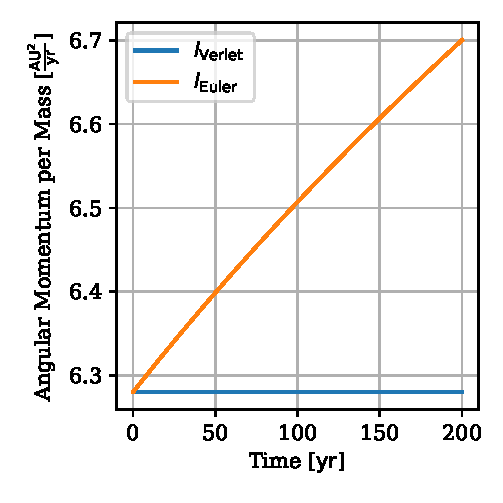
\includegraphics[scale=1]{Figures/taskb_angmom.pdf}
\caption{Angular momentum for Euler and Verlet.}
\label{fig:angmom}
\end{figure}


\begin{figure}
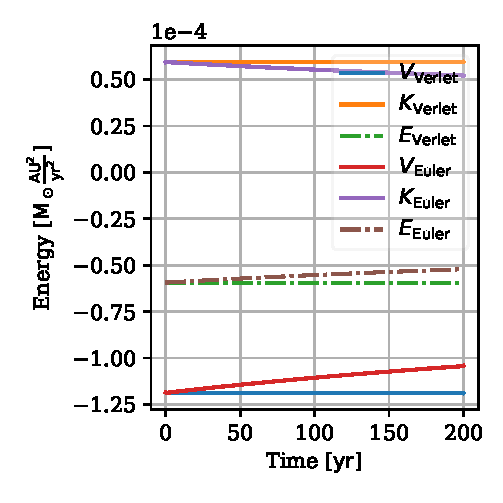
\includegraphics[scale=1]{Figures/taskb_energies.pdf}
\caption{Energies for Euler and Verlet}
\label{fig:energy}
\end{figure}

\begin{figure}
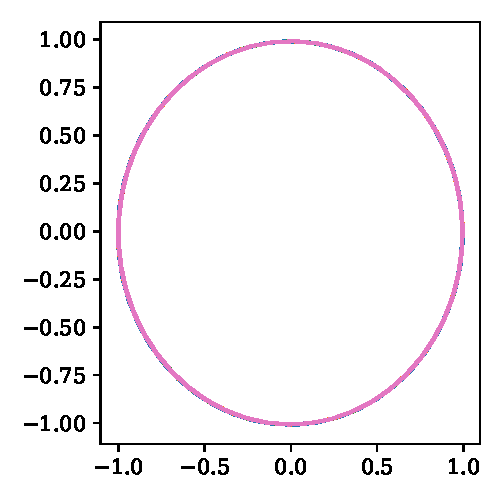
\includegraphics[scale=1]{Figures/taskb_trajectories.pdf}
\caption{Trajectory Sun and Earth}
\label{fig:traj}
\end{figure}

\begin{figure*}
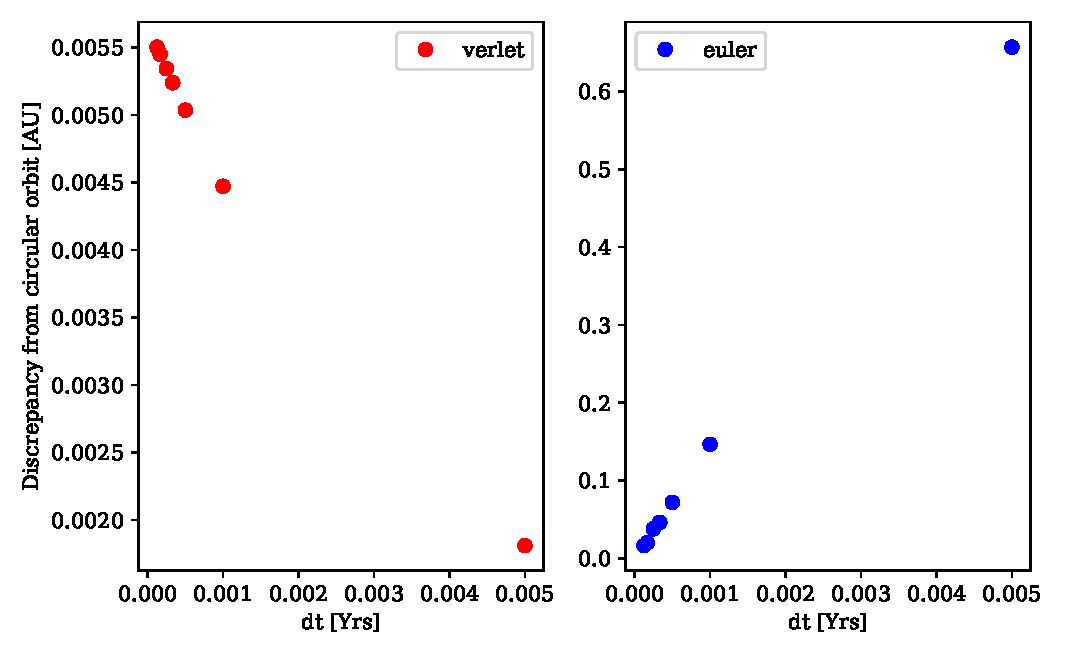
\includegraphics[scale=1]{Figures/taskb_errors.pdf}
\caption{Errors Euler and Verlet}
\label{fig:error}
\end{figure*}

\begin{figure}
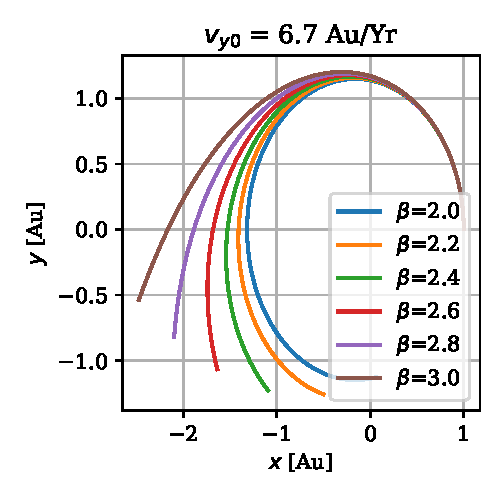
\includegraphics[scale=1]{Figures/beta.pdf}
\caption{Trajectory Earth Sun different $\beta$.}
\label{fig:beta}
\end{figure}

\begin{figure}
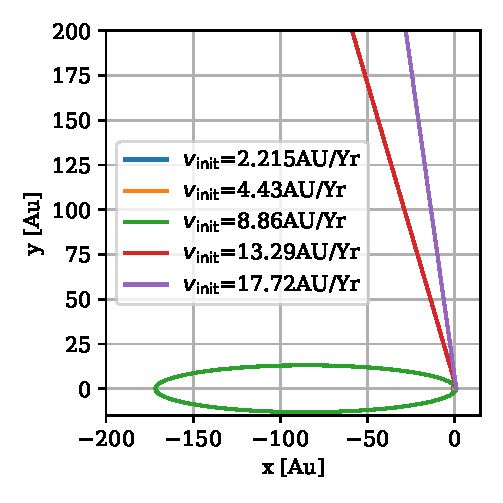
\includegraphics[scale=1]{Figures/espace.pdf}
\caption{Different velocities for Earth Sun system.}
\label{fig:escape}
\end{figure}

\begin{figure}
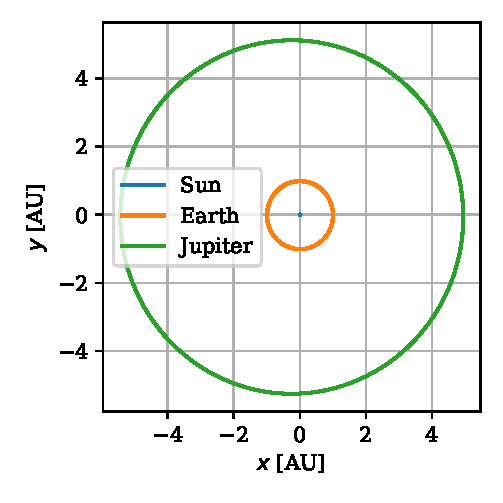
\includegraphics[scale=1]{Figures/jupiter.pdf}
\caption{Jupiter normal weight}
\label{fig:jupiter}
\end{figure}

\begin{figure}
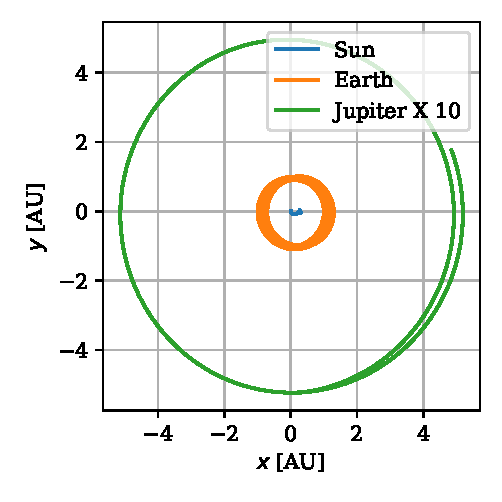
\includegraphics[scale=1]{Figures/jupiter10.pdf}
\caption{Jupiter ten times size}
\label{fig:jupiter10}
\end{figure}

\begin{figure}
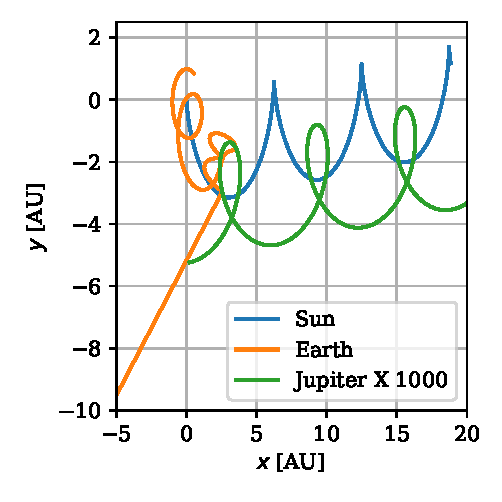
\includegraphics[scale=1]{Figures/jupiter1000.pdf}
\caption{Jupiter 1000 times size}
\label{fig:jupiter1000}
\end{figure}

\begin{figure*}
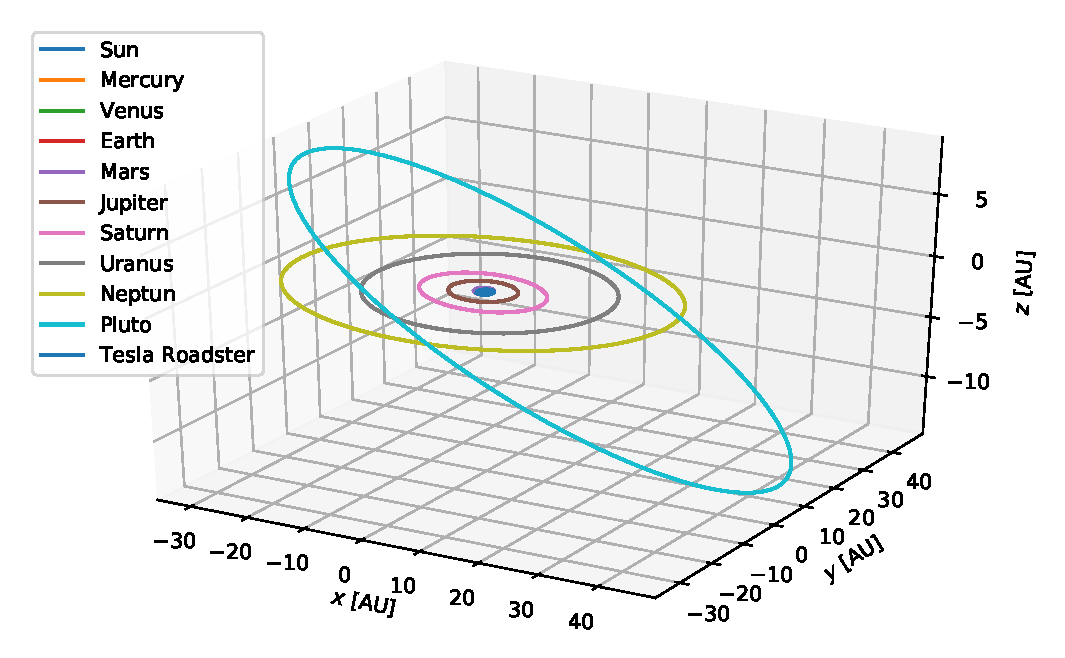
\includegraphics[scale=1]{Figures/OuterSolarSystem.pdf}
\caption{Full solar system}
\label{fig:inner}
\end{figure*}

\begin{figure*}
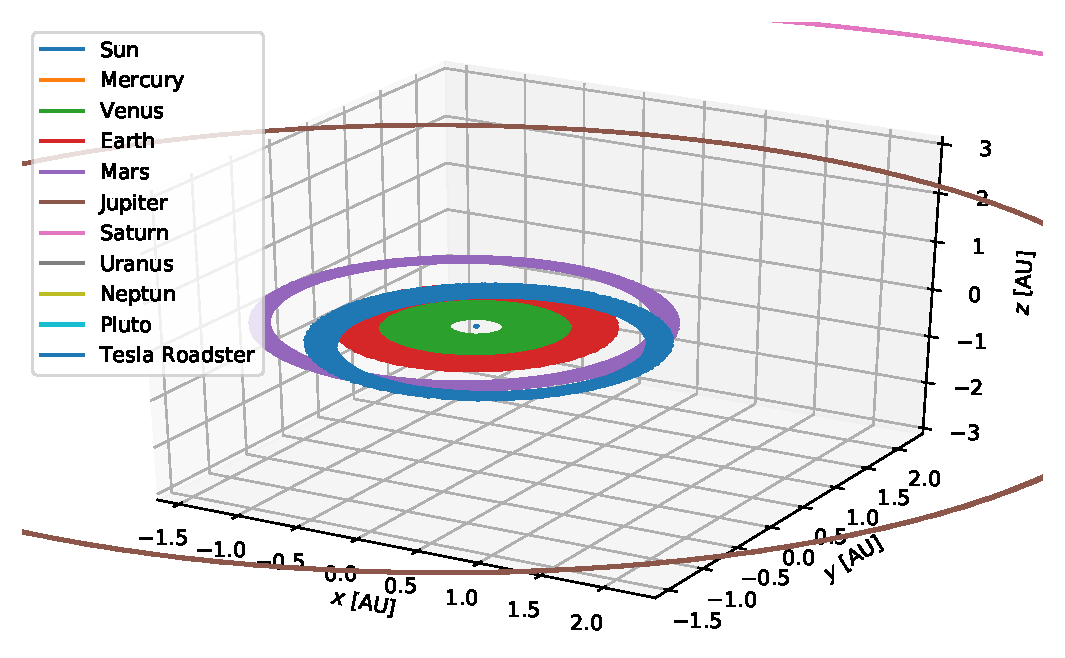
\includegraphics[scale=1]{Figures/InnerSolarSystem.pdf}
\caption{Zoom-in of full solar system}
\label{fig:outer}
\end{figure*}

\section{Discussion} \label{sec:discussion}

\section{Conclusion} \label{sec:conclusion}

\nocite{jensen:2019}
\newpage
\bibliography{ref}
\bibliographystyle{aasjournal}
\end{document}

% End of file `sample62.tex'.
